\section{Codesys}
\thispagestyle{fancy}
\gls{Codesys} \citep{Codesys} laga av \gls{Codesys} Group tilbyr ein open kjeldekodeløysning for prosjeket og har ingen lisenskostnadar. \citep{CodesysLisens}. 
I tillegg så kan prosjektfilene brukast på fleire typar PLS einingar \citep{CodesysPLS}. 
Dette gir vår oppdragsgivar fleksibilitet i korleis dei ønskjer å implementere løysningsforslaget.

\gls{Codesys} nyttar programeringsspråkstandarden satt av \gls{IEC} 61131-3 som omfattar \gls{ST}, ``Sequential Function Chart'' (\gls{SFC}) og ``Ladder Diagram'' (\gls{LD}). 

\gls{Codesys} har nyleg fått støtte for integrering av \gls{github} i programvaren \citep{CodesysGIT}. 
Dette gjer det enklare å halde versjonskontroll og for gruppemedlem å programmere saman. 
\gls{github} har vi nytta på andre prosjekt og det har vi god erfaring med.

Vidare så har \gls{Codesys} støtte for bibliotek gjennom \GLS{Codesys} Store \citep{CodesysStore}. 
Ved å nytte kjende bibliotek, får vi tilgang til ei samling av gjenbrukbare kodeblokker og funksjonar.
Dette er bilbioteka vi ønskjer å nytte

 
\begin{itemize}
    \item \GLS{Codesys} Building Automation \citep{BuildingAutomation}
    \item SysTime \citep{DateAndTime}
    \item Util \citep{Util} \newline \newline
\end{itemize} 

\begin{figure}[htbp]
    \centering
    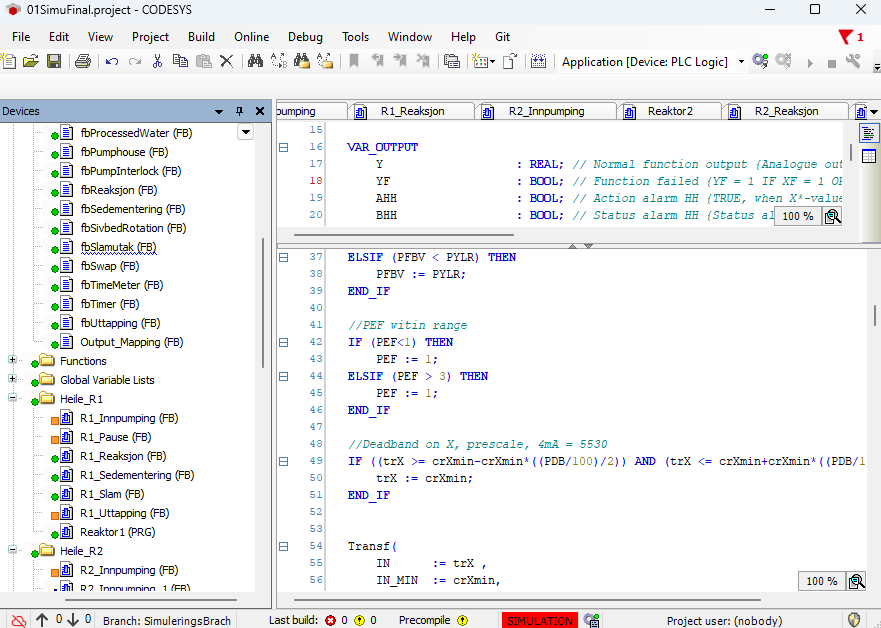
\includegraphics[width=0.6\textwidth]{Bilder/Codesys.png}
    \caption{Codesys programmvare}\label{fig:Codesys}
\end{figure}

\newpage
